\documentclass[11pt]{article}

\usepackage{arxiv}
% Loaded by main.tex
\usepackage[utf8]{inputenc}
\usepackage[T1]{fontenc}
\usepackage{newtxtext}
\usepackage{amsmath,amsthm}
\usepackage{newtxmath}
\usepackage{booktabs}
\usepackage{graphicx}
\usepackage[font=small,labelfont=bf]{caption}
\usepackage{xcolor}
\usepackage[hidelinks]{hyperref}
\usepackage{microtype}
\usepackage[numbers,sort&compress]{natbib}
\bibliographystyle{unsrtnat}
\setlength{\emergencystretch}{2em}
\hypersetup{
  pdftitle={BARCS: beta-binomial regression for multivariable CRISPR screen designs},
  pdfauthor={Hyun-Hwan Jeong},
  pdfsubject={Statistical methods for multivariable CRISPR screens},
  pdfkeywords={CRISPR screen, beta-binomial regression, longitudinal design, calibration}
}

\newcommand{\E}{\operatorname{E}}
\newcommand{\Var}{\operatorname{Var}}
\newcommand{\logit}{\operatorname{logit}}

\definecolor{barcsblue}{HTML}{0072B2}
\definecolor{mageckorange}{HTML}{D55E00}
\definecolor{chronosgreen}{HTML}{009E73}
\definecolor{mageckpink}{HTML}{CC79A7}
\definecolor{bagelgold}{HTML}{E69F00}
\definecolor{waterbearpurple}{HTML}{7A3E9D}
\definecolor{maudered}{HTML}{A33D3D}
\definecolor{naivegray}{HTML}{767676}
\definecolor{cbtwocyan}{HTML}{56B4E9}
\newcommand{\methodswatch}[1]{\textcolor{#1}{\rule{1.1ex}{1.1ex}}}
\newtheorem{lemma}{Lemma}
\newtheorem{proposition}{Proposition}
\newtheorem{corollary}{Corollary}


\shorttitle{BARCS: multivariable beta-binomial regression for CRISPR screens}
\shortauthor{Lee and Jeong}
\title{BARCS: beta-binomial regression for multivariable CRISPR screen analysis}
\author{Kyu-Won Lee\\
\normalsize Baylor College of Medicine\\
\normalsize \texttt{kyuwon.lee@bcm.edu} \\
Hyun-Hwan Jeong\\
\normalsize Baylor College of Medicine\\
\normalsize \texttt{hyun-hwan.jeong@bcm.edu}}
\date{August 2026}

\begin{document}

\maketitle

% !TeX root = ../main.tex
\begin{abstract}
Pooled CRISPR screens increasingly use longitudinal, donor-adjusted, and
factorial designs, but beta-binomial screen methods have largely remained
limited to pairwise comparisons.  BARCS extends the
library-total-conditional beta-binomial model to guide-level regression with
an arbitrary design matrix, so that time, covariate, and interaction effects
can be estimated in a single fit.  In four replicate-complete Cas13 screens,
adding the intermediate time point gave a modest improvement in
essential-gene recovery.  Applying the same non-targeting-control scaling
rule to BARCS, MaGeCK-MLE, edgeR-QL, DESeq2, and limma-voom gave similar
calibration across all five methods, though the four alternatives ranked
essential genes more strongly than BARCS.  In an ordered-bin IL2RA screen,
donor-adjusted BARCS recovered more validated regulators with fewer total
calls than the matched four-bin MAGeCK-MLE fit, and cross-fitted controls
exposed excess guide-level significance.  Simulations showed gains from
dispersion moderation and control-based denominators, but seed-specific
results exposed sensitivity to the denominator choice, and a null grid
traced the large gene-level error to correlated-guide aggregation rather
than to dispersion alone.  Aggregation-matched control scaling reduced this
error but did not remove it.  An external audit of a published beta-binomial
screen showed that the reported CB\textsuperscript{2}
null-discovery count disappeared once full-library totals were restored.
That corrected one denominator-dependent result but did not resolve the
broader calibration concern; nominal-level calibration remains unresolved.
BARCS is a multivariable extension of the beta-binomial CRISPR model, not a
claim of uniform superiority over negative-binomial methods.  Confirmatory
use requires independent biological replication, likelihood-compatible
counts, and held-out or cross-fitted controls.
\end{abstract}


\noindent\textbf{Keywords:} CRISPR screen; beta-binomial regression;
longitudinal design; count data; calibration
\vspace{0.18in}

\section{Introduction}
% !TeX root = ../main.tex
Pooled CRISPR screens increasingly combine time courses, ordered FACS
fractions, donor cohorts, dose series, and factorial treatment arms.  These
experiments ask about slopes, adjusted associations, and interactions.
Reducing them to repeated high-versus-low comparisons discards intermediate
observations and prevents estimation of one effect conditional on the other
design variables.

The count denominator determines how guide abundance is modeled.
Negative-binomial methods generally model marginal counts and account for
library size through normalization or an offset
\citep{marioni2008rnaseq,anders2010deseq,love2014deseq2,lun2016edger}.
In a pooled screen, each guide count is observed together with the total number
of mapped guide reads in its library.  Conditioning on that total treats guide
abundance as a proportion.  A beta-binomial model represents this sampling
structure and separates depth-dependent sequencing variation from
heterogeneity among biological libraries.  The original
CB\textsuperscript{2} study reported better goodness of fit for beta-binomial
than negative-binomial models in pooled CRISPR counts \citep{jeong2019beta}.

CB\textsuperscript{2} applies this principle to two independent groups.
Beta-binomial regression is available in \texttt{corncob} and statistical
packages including \texttt{aod}, \texttt{VGAM}, and \texttt{gamlss}
\citep{martin2020corncob,lesnoff2012aod,yee1996vgam,rigby2005gamlss}, but these
tools lack a CRISPR-oriented workflow connecting full-library totals,
guide-level regression, and screen-level outputs.  Established screen and
RNA-sequencing methods, including MAGeCK-MLE \citep{li2014mageck}, edgeR-QL
\citep{lun2016edger}, DESeq2 \citep{love2014deseq2}, and limma--voom
\citep{law2014voom}, already support multivariable designs.  Chronos and
Waterbear provide specialized models for population dynamics and joint
FACS-bin membership, respectively
\citep{dempster2021chronos,pimentel2024waterbear}.  These methods provide
comparators for assessing the practical value of extending the beta-binomial
screen model.

We developed BARCS (Beta-binomial Analysis and Regression for CRISPR Screens)
to carry the library-total-conditional model into multivariable analysis.
BARCS replaces two group means with a regression design matrix, allowing a
single fit to estimate time, donor-adjusted abundance, treatment, or interaction
effects.  Independent biological libraries determine the residual degrees of
freedom.  Guide-level estimation is followed by optional dispersion moderation,
gene aggregation, and control-based calibration.  The default denominator
retains full-library totals through guide filtering; a separate control-based
normalization option estimates effects relative to a chosen control class.

We first describe the BARCS workflow and evaluate its longitudinal and
covariate-adjusted coefficients in Cas13 and IL2RA screens.  Genome-scale and
factorial simulations then test dispersion moderation and denominator choice
against known truth.  A null-calibration grid examines the consequences of
combining correlated guides, and an external audit assesses the effect of
pre-fit subsetting on a published false-discovery result.  These analyses
establish the uses and limitations of multivariable beta-binomial regression,
including the distinction between recovering biological signals and obtaining
calibrated guide- or gene-level probabilities.


\section{Results}
% !TeX root = ../main.tex
\subsection{BARCS estimates multivariable effects from guide counts}
\label{sec:overview}

BARCS takes a guide-count matrix, library totals, and a sample design matrix.
For guide $g$ in library $i$, the default model is
\begin{equation}
K_{gi}\mid N_i\sim
\operatorname{BetaBinomial}(N_i,\mu_{gi},\rho_g),
\qquad
\logit(\mu_{gi})=\mathbf{x}_i^\top\boldsymbol{\beta}_g,
\label{eq:barcs-model}
\end{equation}
where $N_i$ is the full mapped-guide total before filtering, $\mu_{gi}$ is the
expected guide proportion, and $\rho_g$ represents overdispersion.
The design vector $\mathbf{x}_i$ can contain continuous predictors, group or
donor indicators, and interactions.  A prespecified coefficient or contrast
therefore addresses a question within one joint fit.  BARCS retains the
sampling principle of CB\textsuperscript{2} \citep{jeong2019beta}, with its own
estimation and finite-sample testing procedure.

The workflow fits guide coefficients and dispersion, computes a $t$ statistic
using residual sample degrees of freedom, and summarizes guide evidence when
the reported unit is a gene.  Gene summaries use a directional Stouffer
statistic and the median guide coefficient.  In the simulation ablations,
BARCS-ST uses unmoderated guide statistics and BARCS-MOD applies empirical-Bayes
variance moderation before the same summary.  Real-data analyses use
unmoderated BARCS.  Control scaling adjusts significance without changing
coefficient estimates; its placement is specified for each benchmark.
The Cas13 comparison calibrates gene summaries using aggregation-matched
control pseudo-genes, whereas the IL2RA diagnostic cross-fits a guide-level
scale.  The null simulations below test whether guide-level calibration
extends to gene summaries.

Full-library totals estimate changes in library share.  Control-based
normalization instead expresses abundance relative to a prespecified control
class, as examined in the interaction simulation.  This deliberate change of
reference is distinct from inadvertently recomputing totals after guide
filtering.  The following analyses evaluate the additional design information,
the effects of these optional steps, and the assumptions needed to interpret
the resulting probabilities.

% !TeX root = ../main.tex
% Results subsections, in narrative order.
% !TeX root = ../../main.tex
\subsection{An intermediate Cas13 time point modestly improves recovery}
\label{sec:liang}

The Cas13 fitness screens of \citet{liang2026lncrna} contain measurements at
days 0, 7, and 14.  K562 was excluded because one day-0 replicate was not
deposited.  In HAP1, HEK293FT, MDA-MB-231, and THP1, BARCS, official
MAGeCK-MLE \citep{li2014mageck}, edgeR-QL \citep{lun2016edger}, DESeq2
\citep{love2014deseq2}, and limma--voom \citep{law2014voom} estimated the same
continuous time slope with a replicate block and two-sided tests.

The deposited values had already undergone median-of-ratios normalization,
ComBat correction, and replicate-outlier processing.  We rounded them once to
the nearest pseudo-count and supplied the identical matrix to every method.
This processed-count sensitivity analysis cannot establish how faithfully
either likelihood models raw counts.  Processing can change the effective
depth, as also examined in the external audit.

To test the contribution of the middle time point, we compared the full design
with a BARCS fit using only days 0 and 14.  The three-time-point fit increased
macro-average precision from 0.832 to 0.838 and directional essential-gene
recall at FDR 0.10 from 0.538 to 0.600.  Recall at an empirical 5\% proxy-null
false-positive rate increased from 0.858 to 0.867. The proxy-null $p<0.05$
rate changed from 0.038 to 0.039.  Day 7 therefore modestly improved recovery
with little change in proxy-null rejection.  Cell-line-specific proxy nulls
are targeted lncRNAs with TPM equal to zero in both available expression
assays, so limited expression sensitivity and RfxCas13d collateral activity
can each place a target with a real fitness effect in the null set.  Because
such contamination rewards conservative methods, the proxy-null rates reported
here and in the comparison below are diagnostics rather than validated type-I
errors.

For the head-to-head calibration analysis, the same 1,000 non-targeting guides
were assigned identically to 156--159 pseudo-genes per cell line, with guide
counts sampled from the target-gene distribution.  We applied the same
tail-scaling rule to each method's native pseudo-gene summary.  Mean
cell-line-specific absolute calibration error was 0.0207 for BARCS, 0.0198 for
DESeq2, 0.0181 for edgeR-QL, 0.0178 for limma--voom, and 0.0171 for
MAGeCK-MLE.  The calibration diagnostics were therefore similar after the
common scaling rule.  The four alternatives ranked known essential genes more
strongly.  Average precision was 0.838 for BARCS and 0.874--0.877 for the four
alternatives; directional recall at gene FDR 0.10 was 0.600 versus
0.738--0.767.  At a matched empirical 5\% proxy-null rate, recall was 0.867
versus 0.879--0.888.

\begin{figure}[!htbp]
\centering
\includegraphics[width=\textwidth]{figures/liang_longitudinal_volcano_trajectories.pdf}
\caption{\textbf{Longitudinal Cas13 sensitivity analysis using days 0, 7, and
14.}  (A--E) Gene-level results for BARCS, MAGeCK-MLE, edgeR-QL, DESeq2, and
limma--voom across the four replicate-complete cell lines.  All five panels
use common axis scales to display the method-specific effect estimates.  The x axis is the signed logarithmic transform
$\mathrm{sign}(\beta)\log_{10}(1+|\beta|/0.25)$, labelled at the untransformed
effect values.  The horizontal line marks two-sided $p=0.05$; $-\log_{10}(p)$
is clipped at 60.  Triangles mark clipped points, whose count is shown above
each panel.  Colour denotes cell line
throughout the figure; coloured points are negative-effect genes called at FDR
0.10, and all remaining genes are grey.  (F--H) Processed guide abundance in
counts per million for three proxy-null disagreements, with markers filled by
cell line and replicates distinguished by point shape and line type.  Among
proxy-null
guides, 61 satisfied BARCS $p\geq0.20$ with all three guide-level alternatives
$p<0.05$.  Within each cell line, the candidate minimizing the largest
alternative $p$ was identified; the three with the largest ratio of BARCS
$p$ to that maximum are displayed.  Conversely, 1,242 proxy-null guides had
BARCS $p<0.05$ while all three alternatives had $p\geq0.05$.  The panels show trajectories selected from one direction of disagreement; they
do not estimate its prevalence.}
\label{fig:liang}
\end{figure}

Figure~\ref{fig:liang} pairs the gene-level comparison with three guide
trajectories selected by the stated disagreement rule, showing the time
patterns behind those differences in significance.

\FloatBarrier

% !TeX root = ../../main.tex
\subsection{A covariate-adjusted ordered phenotype recovers validated
regulators}
\label{sec:facs}

We next asked whether the design-matrix extension is useful outside a time
course.  GSE242880 contains an IL2RA protein-abundance screen in primary human
T cells, with four ordered FACS bins for each of three donors, 6,000 guides,
and 26 regulators validated by individual knockout and flow cytometry
\citep{freimer2022il2ra,pimentel2024waterbear}.  The four bins were assigned
prespecified latent normal locations, and BARCS fitted one marker-abundance
slope with donor indicators.  Official MAGeCK-MLE received the same design.
All comparisons below used all four ordered fractions.

This experiment also provides a direct model diagnostic.  Bins from one donor
partition the same cell pool and are negatively dependent, whereas the
guide-level BARCS fit treats their margins independently.  Among 593
non-targeting guides, the uncalibrated $p<0.05$ frequency was 0.133.  Because
\texttt{bb\_calibrate\_controls()} estimates its scale from the control tail,
evaluating those same guides after fitting would be circular.  We therefore
used deterministic five-fold cross-fitting: each guide was evaluated with a
scale estimated from the other four folds.  The held-out $p<0.05$ rate was
29/593 (0.049).  Fold-specific scales ranged from 1.332 to 1.418.  A
prespecified seeded permutation of the guide-to-fold assignment gave 31/593
(0.052), with scales from 1.332 to 1.417, arguing against structure induced by
guide-identifier ordering.  The production gene analysis used all controls to
estimate one scale; calibration does not change effect estimates or their
ranking.

\begin{table}[htbp]
\centering
\caption{Ordered-bin IL2RA sensitivity analysis.  Recovery requires a
discovery at each method's threshold and the experimentally validated
direction; all rows use all four FACS bins.  The BARCS NTC rate is five-fold
held out; it is not measured on the
controls used to estimate that fold's scale.  ``Validated'' is the number of
the 26 experimentally validated regulators recovered in the validated
direction.  ``Panel hits/call'' divides that number by all method calls.  It
describes how concentrated a call set is around this limited validation panel;
it is not statistical precision or the probability that an individual call is
true, because genes outside the panel were not individually validated.  An em
dash indicates that a comparable guide-level NTC rate was not available.}
\label{tab:waterbear}
\small
\setlength{\tabcolsep}{4pt}
\begin{tabular}{lrrrr}
\toprule
Method & Discoveries & Validated & Panel hits/call & NTC $p<0.05$\\
\midrule
\methodswatch{barcsblue} BARCS, calibrated &
49 & 22/26 & 22/49 (44.9\%) & 0.049\\
\methodswatch{barcsblue} BARCS, raw &
127 & 23/26 & 23/127 (18.1\%) & 0.133\\
\methodswatch{mageckorange} MAGeCK-MLE &
72 & 17/26 & 17/72 (23.6\%) & ---\\
\methodswatch{waterbearpurple} Waterbear \citep{pimentel2024waterbear} &
79 & 24/26 & 24/79 (30.4\%) & ---\\
\methodswatch{maudered} MAUDE \citep{deboer2020maude} &
406 & 25/26 & 25/406 (6.2\%) & ---\\
\bottomrule
\end{tabular}
\end{table}

Control-calibrated BARCS recovered 22 of 26 validated regulators with 49
discoveries, compared with 17 of 26 and 72 discoveries for the matched
MAGeCK-MLE fit (Table~\ref{tab:waterbear}).  This corresponds to validation
panel-hit fractions of 44.9\% and 23.6\%, respectively; these fractions do not
classify the remaining calls as false.  Relative to raw four-bin BARCS,
control calibration reduced the call set from 127 to 49 while retaining 22 of
the 23 validated regulators recovered by the raw analysis.  The held-out NTC
rate simultaneously moved from 0.133 to 0.049, showing why the calibrated
four-bin result is the primary BARCS operating point.

The specialist models remain important comparators.  Waterbear recovered 24
validated regulators and MAUDE recovered 25, but with 79 and 406 discoveries.
BARCS therefore offered the strongest recovery-per-discovery ratio among the
four-bin models shown, while Waterbear remained the more faithful generative
model for correlated sorted bins.  Negative controls diagnose the independence
violation and calibrate one operating point; they do not make the bin margins
independent.

% !TeX root = ../../main.tex
\subsection{Dispersion moderation improves BARCS in genome-scale simulation}
\label{sec:crispulator}

We used CRISPulator to evaluate a FACS design under known truth
\citep{nagy2017crispulator}.  At the primary multiplicity of infection
(MOI) of 0.20, three prespecified seeds each generated 10,000 genes, five
guides per gene, four independent replicates, and low, bulk, and high
fractions.  All methods received the same counts and design.

The BARCS comparison isolates guide-dispersion moderation.  BARCS-ST uses the original
guide-specific dispersion estimate, whereas BARCS-MOD moderates those
estimates before applying the same gene summary.  Moderation increased average
precision from 0.902 to 0.919 and F1 at gene FDR 0.10 from 0.811 to 0.847,
while realized FDP remained nearly unchanged (0.065 and 0.066).  This supports
dispersion moderation within the common BARCS pipeline.

\begin{table}[htbp]
\centering
\caption{Genome-scale CRISPulator comparison for the primary three-bin design
at MOI 0.20 (three-seed mean).  Each method
is evaluated at its nominal gene-level threshold; the resulting operating
points are therefore not matched on realized FDP.}
\label{tab:crispulator-comparators}
\small
\begin{tabular}{lrrrr}
\toprule
Method & AUROC & Average precision & Realized FDP & F1\\
\midrule
BARCS-ST & 0.947 & 0.902 & 0.065 & 0.811\\
BARCS-MOD & 0.954 & 0.919 & 0.066 & 0.847\\
MAGeCK-MLE & 0.957 & 0.921 & 0.006 & 0.718\\
CRISPhieRmix & 0.929 & 0.867 & 0.197 & 0.785\\
\bottomrule
\end{tabular}
\end{table}

\begin{figure}[!t]
\centering
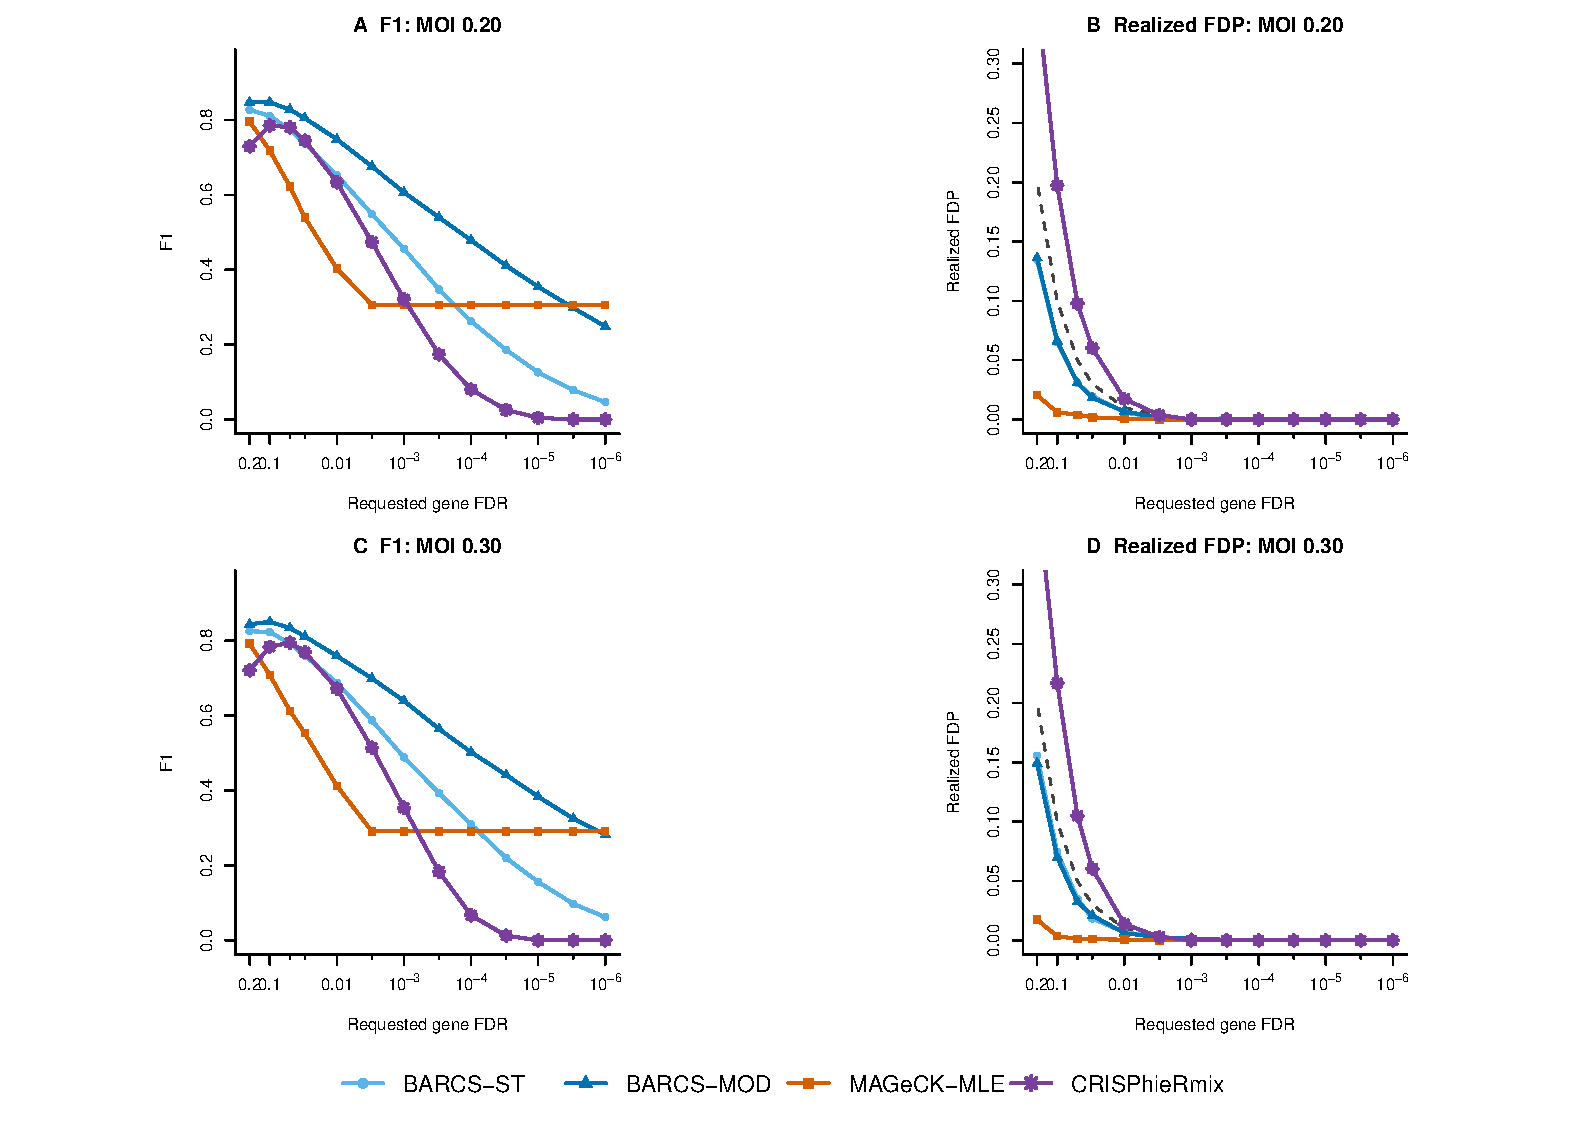
\includegraphics[width=\textwidth]{figures/crispulator_facs_moi_10k_f1_by_fdr.pdf}
\caption{\textbf{CRISPulator threshold sensitivity.}  (A,B) MOI 0.20 and
(C,D) MOI 0.30.  F1 is shown on the left and realized FDP on the right; the
dashed diagonal denotes realized FDP equal to the nominal threshold.  F1 panels use a common y scale, as do realized-FDP panels.
All 13 evaluated thresholds are marked.  BARCS-ST and BARCS-MOD are two settings of one estimator and
therefore share a colour, separated by line type and point shape.  The shared
simulation, gene summary, and thresholds isolate the BARCS-ST versus BARCS-MOD
moderation effect.}
\label{fig:crispulator}
\end{figure}

The moderation gain persisted across requested thresholds at MOI 0.20 and in
the secondary MOI-0.30 analysis (Figure~\ref{fig:crispulator}).  Fitting the
50,000 guide-level regressions required 70.1--102.8 seconds per primary seed
on the analysis system, providing a direct screen-scale runtime check.
MAGeCK-MLE slightly exceeded BARCS-MOD in AUROC and average precision while
operating at a much lower realized FDP; CRISPhieRmix operated at a higher FDP
(Table~\ref{tab:crispulator-comparators}).  These differences limit
comparisons of F1 at a common nominal threshold.  In the broader 400-gene
comparison, edgeR-QL, DESeq2, and limma--voom matched or exceeded BARCS
ranking.  After matching methods on realized FDP, the comparison did not
distinguish the methods above an FDP of 0.005.

% !TeX root = ../../main.tex
\subsection{Control denominators recover interactions under composition shifts}
\label{sec:simcrispr}

We used simCRISPR to generate a factorial knockout-by-treatment screen with a
known guide-level interaction \citep{zhu2026simcrispr}.  Each of three seeds
contained 2,000 sgRNAs and three independent replicates per factorial arm.
Non-targeting guides had a true interaction of zero, and safe-harbor guides
separated the effect of cutting from a targeted gene effect.  Each control
class was split so that normalization and calibration guides were never used
for evaluation.  The benchmark compares denominator choice and moderation
within BARCS. MAGeCK-MLE is a reference with one guide per gene, an input that
lacks within-gene replication for its native gene model and cannot support a
method ranking.

\begin{table}[ht]
\centering
\caption{Interaction recovery in simCRISPR (three-seed mean with standard
deviation in parentheses).  Recall and F1
use targeting guides with $|\mathrm{interaction}|\geq0.2$ as positives.  Null
and safe-harbor rates are held-out call fractions at FDR 0.10.}
\label{tab:simcrispr}
\scriptsize
\setlength{\tabcolsep}{2.5pt}
\begin{tabular}{llrrrr}
\toprule
Method & Denominator & Dir.\ recall & F1 & Null rate & Safe-harbor\\
\midrule
BARCS-ST & Library &
0.376 (0.308) & 0.488 (0.389) & 0.004 (0.008) & 0.002 (0.003)\\
BARCS-MOD & Library &
0.375 (0.323) & 0.481 (0.409) & 0.000 (0.000) & 0.000 (0.000)\\
\midrule
BARCS-ST & Non-targeting &
0.769 (0.094) & 0.870 (0.065) & 0.024 (0.020) & 0.070 (0.025)\\
BARCS-MOD & Non-targeting &
0.838 (0.025) & 0.917 (0.017) & 0.040 (0.040) & 0.080 (0.038)\\
\midrule
BARCS-ST & Safe-harbor &
0.762 (0.087) & 0.864 (0.061) & 0.042 (0.027) & 0.042 (0.008)\\
BARCS-MOD & Safe-harbor &
0.830 (0.019) & 0.914 (0.017) & 0.027 (0.023) &
0.035 (0.005)\\
\midrule
MAGeCK-MLE & Non-targeting &
0.003 (0.001) & 0.006 (0.002) & 0.000 (0.000) & 0.000 (0.000)\\
\bottomrule
\end{tabular}
\end{table}

The full-library denominator preserved effect ranking but shifted the
true-zero guides because widespread depletion increased every surviving
guide's library share.  Their median fitted interaction was 0.184
(interquartile range 0.136--0.231), whereas the corresponding medians were
0.004 and 0.030 for the non-targeting and safe-harbor denominators.  The
control-scale factors were 1.99 and 2.24 for unmoderated and moderated
full-library fits, compared with 1.00--1.07 for the control-denominator fits.
One library-denominator seed collapsed, so the three-seed means in
Table~\ref{tab:simcrispr} poorly describe a typical run.  BARCS-ST F1 was
0.039, 0.709, and 0.716 across the three seeds; BARCS-MOD F1 was 0.011, 0.680,
and 0.754.  With the non-targeting denominator, the corresponding values were
0.798, 0.924, and 0.889 for BARCS-ST and 0.899, 0.933, and 0.920 for
BARCS-MOD. The control denominator improved every seed, with gains that varied
across runs.  In the two noncollapsed runs, F1 was approximately 0.71 versus
0.91, a smaller gain than a near doubling.  The held-out null rates remained
below the nominal 0.10 in all cases.

\begin{figure}[!htbp]
\centering
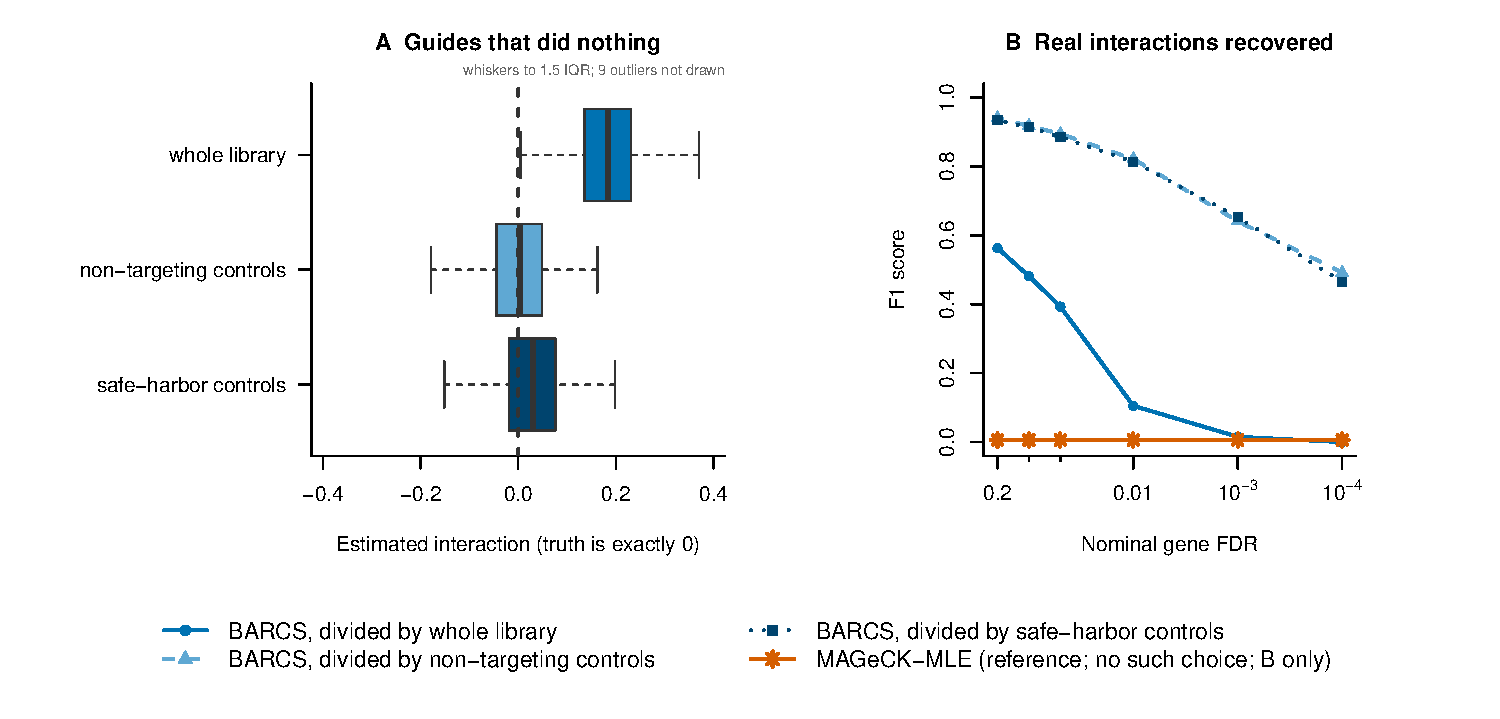
\includegraphics[width=\textwidth]{figures/simcrispr_interaction.pdf}
\caption{\textbf{Denominator choice controls interaction recovery.}  (A)
Estimated interactions among true-zero guides.  A full-library denominator
induces a positive shift; either control denominator removes it.  Boxes span
the interquartile range, whiskers extend to 1.5 times it, and the panel reports the number of observations beyond the whiskers without
plotting those points.
(B) F1 across nominal FDR thresholds; every evaluated threshold is marked.  Control denominators retain
substantially more interaction power.  The three denominator settings share a hue and differ in lightness, line type,
and point shape.  MAGeCK-MLE uses its colour from the other figures and
appears only in (B).}
\label{fig:simcrispr}
\end{figure}

Figure~\ref{fig:simcrispr} shows the composition-induced null shift and
threshold curves.  Although the control denominators performed similarly
overall, they differed in their handling of cutting artifacts.  Safe-harbor
guides were called at 0.080 after non-targeting normalization and 0.035 after
safe-harbor normalization. In these simulations, both control classes
supported targeted-interaction recovery, while safe-harbor normalization
absorbed more of the shared cutting response.  A comparison of gene-level
interaction methods would require several independently simulated guides per
gene and a common gene-level interaction estimand.

% !TeX root = ../../main.tex
\subsection{Denominator correction removes one artifact but does not resolve
calibration}
\label{sec:supp-fdr-audit}

The recent false-discovery manuscript by \citet{dempster2025fdr} raised the
concern that CB\textsuperscript{2}, and beta-binomial CRISPR analysis more
broadly, could be anti-conservative.  H.-H.J.\ also developed
CB\textsuperscript{2}, so this reanalysis audits an author's prior method and
is not an independent assessment.  We revisited its deposited benchmark
\citep{dempster2025fdrdata} to distinguish the effects of the sampling model
from those of input preparation.  The benchmark compared
CB\textsuperscript{2}, MAGeCK \citep{li2014mageck}, JACKS
\citep{allen2019jacks}, DrugZ \citep{colic2019drugz}, and Chronos.  For Avana,
we re-evaluated the published CB\textsuperscript{2} analysis
\citep{jeong2019beta} after restoring the full-library denominator; BARCS was
not fitted because this audit isolates the denominator used by
CB\textsuperscript{2}.  For PSN1 and DeWeirdt, we retained the deposited
CB\textsuperscript{2} results and ran BARCS on the deposited normalized
tables.  The DeWeirdt analysis used Fisher aggregation of guide probabilities
to form gene summaries.  In the reported Avana analysis, restriction to null
genes before fitting changed the column totals.  Reusing the full-library
CB\textsuperscript{2} probabilities for the same genes reduced the number of
FDR 0.10 discoveries from 152 to zero.  The 152-call result therefore depended
on the fitted denominator.  The broader concern about anti-conservative
beta-binomial analyses remains.

\begin{table}[htbp]
\centering
\caption{Expected and observed behavior in the external false-discovery audit.
Reported results and deposited inputs follow \citet{dempster2025fdr} and the
accompanying data release \citep{dempster2025fdrdata}.  For an all-null
benchmark, a well-calibrated analysis should produce approximately uniform
null $p$-values, about 5\% below 0.05, and few or no calls after FDR control.
For DeWeirdt, ``known'' denotes 28 curated condition--gene combinations
\citep{deweirdt2020isogenic}, not a complete truth set; therefore no exact
number of expected calls can be specified.}
\label{tab:chronosaudit}
\footnotesize
\setlength{\tabcolsep}{3pt}
\renewcommand{\arraystretch}{1.10}
\begin{tabular}{>{\raggedright\arraybackslash}p{0.14\textwidth}
                >{\raggedright\arraybackslash}p{0.24\textwidth}
                >{\raggedright\arraybackslash}p{0.34\textwidth}
                >{\raggedright\arraybackslash}p{0.19\textwidth}}
\toprule
Benchmark & Expected if the analysis is well behaved & Observed result &
Interpretation\\
\midrule
Avana null-only &
Approximately 5\% of null $p$-values below 0.05; few or no calls at FDR 0.10 &
Reported CB\textsuperscript{2}: 152 calls at FDR 0.10.  Full-total
CB\textsuperscript{2}: 0 calls.  BARCS was not run &
The 152-call result was denominator-dependent; the residual null rate of 0.145
leaves the broader miscalibration concern unresolved\\
\addlinespace[2pt]
PSN1 null split &
Held-out guide $p<0.05$ rate near 0.05, control scale near 1, and few or no
gene calls &
Reported CB\textsuperscript{2}: 0 gene calls.  BARCS: 0 gene calls; guide
$p<0.05$ rates 0.0481 raw and 0.0465 scaled; control scale 1.017 &
This result is consistent with the null expectation, but one benchmark does
not establish general calibration\\
\addlinespace[2pt]
DeWeirdt differential screens &
Known interactions enriched among calls, with no comparison dominating solely
because of a quality artifact &
Reported CB\textsuperscript{2}: 0 calls and 0/28 known recovered.  BARCS: 38
calls and 1/28 known recovered; 37/38 calls arose in one comparison &
Poor known-interaction recovery and one-comparison concentration suggest
comparison-specific confounding\\
\bottomrule
\end{tabular}
\end{table}

In PSN1, BARCS pooled one dispersion estimate per guide across the design and
retained a near-nominal guide null rate (Table~\ref{tab:chronosaudit}).  In
the DeWeirdt screens \citep{deweirdt2020isogenic}, however, BARCS recovered
only MCL1 under A-1331852; 37 of its 38 calls came from the OVCAR8--olaparib
comparison without recovering BRCA1 or BRCA2.  With only two replicates per
arm, treatment-associated quality shifts remain a possible explanation for
this concentration of calls.

The concern raised by \citet{dempster2025fdr} remains, although the 152-call
example also depends on input preparation.  Pre-fit guide subsetting and
common normalization can alter the effective depth in a
library-total-conditional model.  Zero Avana discoveries after restoring the
full total do not demonstrate nominal calibration: the largest
cell-line-specific $p<0.05$ rate remained 0.145, and the DeWeirdt analysis
remained unstable.  Comparator studies must preserve full-library totals,
separate calibration guides from evaluation guides, and use blocked
permutations or independent validation for differential screens.



\section{Discussion}
% !TeX root = ../main.tex
BARCS fits time courses, covariate-adjusted effects, and factorial
interactions through a common beta-binomial regression interface.  The
library-total-conditional model specifies the denominator, and control
diagnostics assess calibration.  The sampling model determines how sequencing
depth and between-library variation enter the fit; the design matrix
determines which biological question the coefficient addresses.

In Cas13, adding the intermediate time point improved essential-gene recovery
modestly.  All four alternative methods ranked essential genes more strongly,
however, and aggregation-matched control scaling produced similar calibration
diagnostics across methods.  Because the input was normalized and
ComBat-corrected, this comparison provides limited evidence about the
underlying count likelihoods.  In IL2RA, donor-adjusted BARCS recovered more
validated regulators with fewer calls than the matched MAGeCK-MLE fit.
Waterbear and MAUDE recovered more members of the validation panel, and the
panel's limited coverage prevents interpreting recovery per call as positive
predictive value.

In the simulations, moderation improved genome-scale F1, although MAGeCK-MLE
retained slightly stronger ranking and a lower realized FDP.  Control-based
denominators improved interaction recovery in every simulated seed, with a
much larger gain in the one seed where the full-library fit collapsed.  These
denominator choices change the reference for abundance: full-library effects
describe changes in library share, whereas control-based effects describe
changes relative to the selected control class.  Non-targeting and safe-harbor
controls also differ in whether they absorb the shared cutting response.  The
appropriate control class depends on the effect being estimated and the
behavior of the controls.

The IL2RA cross-fitting analysis supports the guide-level operating point
examined here.  The null grid shows why that result cannot establish
gene-level calibration: correlated guides can inflate Stouffer gene
probabilities even when guide tests appear calibrated.  Scaling after matched
aggregation reduced this inflation but left appreciable error in some cells.
The beta-binomial fit also uses plug-in dispersion estimates; a residual-$t$
reference does not fully account for their uncertainty.  Nominal gene-level
FDR thresholds in these analyses therefore lack a general calibration
guarantee.  Further development should account for guide dependence in gene
aggregation and assess calibration using blocked permutations or independent
controls.

In the external audit, restoring full-library totals corrected the reported
Avana CB\textsuperscript{2} discovery count, but the residual null inflation
and poor DeWeirdt interaction recovery leave the broader calibration concern
intact. Preserving totals through filtering prevents an unintended change in
the model; it does not resolve the effects of dependence, processed counts, or
comparison-specific confounding.

BARCS is most directly interpretable with likelihood-compatible counts and
independent biological libraries.  Repeated harvests from one culture and FACS
bins partitioned from one donor require repeated-measures or joint models to
represent their dependence.  Donor indicators adjust mean differences but do
not supply that covariance structure.  For these designs, the fitted
coefficients and control diagnostics remain exploratory.  Confirmatory
applications require biological replication and calibration checks at the
guide or gene level used to report discoveries.


\section{Methods}
% !TeX root = ../main.tex
\subsection{Model and inference}

For guide $g$ in library $i$, BARCS models the count conditional on the
unfiltered mapped-guide total:
\begin{equation}
K_{gi}\mid N_i\sim
\operatorname{BetaBinomial}(N_i,\mu_{gi},\rho_g),
\qquad
\logit(\mu_{gi})=\mathbf{x}_i^\top\boldsymbol{\beta}_g .
\label{eq:barcs-model}
\end{equation}
The coefficient model in Equation~\eqref{eq:barcs-model} allows the design
vector to contain time, dose, donor, batch, treatment, and
interaction terms.  Coefficients are estimated by beta-binomial weighted
logistic regression.  A prespecified coefficient or contrast is divided by
its model-based standard error and compared with a Student $t$ distribution
using residual sample degrees of freedom.  All reported tests are two-sided,
and guide- or gene-level probabilities are adjusted by Benjamini--Hochberg.
The guide-specific overdispersion $\rho_g$ is estimated by solving the Pearson
equation at the fitted mean, truncated at zero when the counts are not
overdispersed, and the coefficient and dispersion updates are alternated to
convergence.  BARCS-ST reports these unmoderated statistics.  BARCS-MOD
additionally shrinks each guide's fitted variance toward a trend in log mean
abundance by an empirical-Bayes step that changes standard errors and residual
degrees of freedom but not the coefficient estimates; the real-data benchmarks
use unmoderated BARCS.  The full estimating equations are given in the
Supplement.

\subsection{Gene-level aggregation and control calibration}

Guide coefficients are combined into a gene-level statistic by a prespecified
directional Stouffer summary: each guide's two-sided probability is converted
to a normal deviate carrying the sign of its coefficient, the deviates for a
gene are combined by the Stouffer rule, and the result is returned to a
two-sided gene probability, which is then adjusted by Benjamini--Hochberg.  The
reported gene effect is the median guide coefficient.

Control calibration rescales a reported statistic without altering the
coefficient estimates or their ranking.  Given a set of negative-control
features, \texttt{bb\_calibrate\_controls()} maps the 95th percentile of the
absolute signed-normal control statistic onto the two-sided standard-normal
0.05 cutoff and divides by the resulting scale, with scales below one truncated
at one so that the adjustment can only be conservative.  Two properties matter
for interpretation.  First, the scale must be estimated at the same aggregation
level as the statistic it corrects, because a scale learned from individual
control guides does not transfer to multi-guide gene statistics; non-targeting
guides are therefore grouped into pseudo-genes matching the target-gene
guide-count distribution before the rule is applied to a gene-level summary.
Second, the controls used to estimate the scale cannot also be used to evaluate
it.  Wherever a control-based error rate is reported, the scale is obtained by
deterministic five-fold cross-fitting and each fold is evaluated with the scale
estimated from the other four.

\paragraph{Validity of gene-level probabilities.}
The directional Stouffer summary treats the guides of a gene as independent
sources of evidence.  Guides targeting the same gene are generally positively
correlated---through a shared target effect, a shared cutting response,
copy-number-associated toxicity, clonal structure, or unmodeled library
composition shifts---and under positive correlation the combined statistic is
anti-conservative; the null-calibration grid in the Supplement quantifies the
resulting gene-level error.  Gene-level probabilities are therefore reported as
empirically calibrated ranking statistics rather than as tests carrying a
nominal false-discovery guarantee.  Guide-level coefficients, their standard
errors, and their ordering are unaffected by this limitation, and gene-level
inference is recovered when the gene-level null is established by permutation
that preserves the within-gene guide structure and the experimental blocking.

\subsection{Denominator choice defines the estimand}

The two denominators available in BARCS answer different questions and are not
interchangeable.  Under the full-library total, $\beta$ is the change in a
guide's share of the sequenced library.  This quantity is always well defined,
but it coincides with the change in absolute guide abundance only when the
overall library composition is stable across the design; when a large fraction
of guides deplete, every surviving guide's share rises and true-null guides
acquire a positive shift (Figure~\ref{fig:simcrispr}).  Under a control-set
denominator, $\beta$ is the change relative to that control set, and it
identifies the absolute effect under the assumption that the control set is
invariant across design levels.  That assumption should be checked rather than
assumed, by comparing the control set's share of the library across design
levels.  Non-targeting controls are the efficient choice when the quantity of
interest is a targeted effect; safe-harbor controls additionally absorb the
shared cutting response and are preferred in Cas9 knockout screens with
widespread depletion.

\subsection{Longitudinal Cas13 analysis}

For HAP1, HEK293FT, MDA-MB-231, and THP1, days 0, 7, and 14 were fitted
jointly with continuous time and a replicate indicator.  K562 was excluded
because one day-0 replicate was absent.  BARCS, MAGeCK-MLE, edgeR-QL, DESeq2,
and limma--voom received the identical rounded matrix and tested the same time
slope.  Non-targeting guides were grouped into pseudo-genes matching the
target-gene guide-count distribution, and the same post-aggregation control
scaling rule was applied to all five methods.  A BARCS endpoint fit using only
days 0 and 14 tested the value of the intermediate time point.  Known
essential genes were positives; targeted lncRNAs with TPM equal to zero in
both available expression assays were proxy nulls.  That definition is
imperfect in a direction that favours conservative methods, so the proxy-null
rates are diagnostics rather than validated type-I errors.  Because the deposited values were already normalized and
ComBat-corrected, this analysis was treated as a processed-count sensitivity
study.

\subsection{Ordered-bin IL2RA analysis}

The IL2RA screen comprised four ordered FACS bins from each of three donors.
BARCS fitted one ordered-bin score with donor indicators, and MAGeCK-MLE
received the same design.  Of 593 non-targeting guides, four folds estimated
the control scale and the omitted fold evaluated it; this was repeated across
five deterministic folds.  A seeded permutation of fold assignments checked
that identifier ordering did not determine the result.  Method discoveries
were compared with 26 regulators
validated by individual knockout and flow cytometry.  Waterbear and MAUDE
results were taken from their published analyses of the same experiment.

\subsection{Simulation benchmarks}

CRISPulator generated three 10,000-gene FACS screens with five guides per gene
and four independent replicates.  BARCS-ST and BARCS-MOD differed only by
guide-dispersion moderation.  simCRISPR generated three factorial
knockout-by-treatment screens with 2,000 sgRNAs and three replicates per arm.
Its known interaction effects allowed direct comparison of full-library,
non-targeting, and safe-harbor denominators.  Control guides used for
normalization and calibration were held out from scoring.

\subsection{External and supplementary analyses}

The external false-discovery audit re-evaluated the deposited Avana
CB\textsuperscript{2} probabilities using full-library totals and ran BARCS on
the deposited PSN1 and DeWeirdt normalized tables.  Supplementary analyses
include the serial-harvest HT-29 screen, a four-coefficient GSE70038 screen
with method-specific pathway enrichment, and the Sanson A375 endpoint and
copy-number audit.  The Supplement reports their complete preprocessing,
design, and scoring definitions in the same order as the corresponding
results.


% !TeX root = ../main.tex

\section*{Author contributions}
\textbf{[TO COMPLETE BEFORE SUBMISSION]} State each author's contribution.
CRediT-style attribution when there is more than one
author, drawn from conceptualization, methodology, software, validation, formal
analysis, investigation, data curation, writing---original draft,
writing---review and editing, visualization, supervision, project
administration, and funding acquisition.

\section*{Funding}
\textbf{[TO COMPLETE BEFORE SUBMISSION]} List funding sources and grant
numbers, or state explicitly that this work received no specific funding.

\section*{Competing interests}
\textbf{[I know this part was removed intentionally before, but adding it as claude suggestion.]} Declare any further
competing interests, or state that there are none. H.-H.J.\ is an author of CB\textsuperscript{2}, the two-group beta-binomial
screen method that BARCS extends and whose published Avana analysis is
re-evaluated in the external false-discovery audit reported here. That
re-evaluation is therefore an audit of a method developed by one of the present
authors rather than an independent adjudication, as stated in the corresponding
Results section.

\section*{Data availability}
Every dataset analysed in this study is publicly available and no new primary
data were generated.  The longitudinal Cas13 fitness screens are the deposited
supplementary tables of \citet{liang2026lncrna}; the corresponding raw
sequencing reads are in the NCBI Sequence Read Archive under BioProject
accession PRJNA1344834, for which a restartable read-processing pipeline is
included with the analysis code.  The ordered-bin IL2RA screen is in the NCBI
Gene Expression Omnibus under accession GSE242880
\citep{pimentel2024waterbear}, and the 26 individually validated regulators
used as the recovery panel are those reported by \citet{freimer2022il2ra}.

The supplementary benchmarks reuse three further public screens.  The
longitudinal HT-29 time course is Data S2 of \citet{tzelepis2016dropout},
obtained through the Europe PMC supplementary bundle for PMC5081405.  The
Brunello A375 endpoint screen is the count table distributed with
CB\textsuperscript{2} \citep{jeong2019beta}, originally reported by
\citet{sanson2018optimized}, with the reference essential and nonessential
gene sets of \citet{hart2017evaluation}.  The four-coefficient multivariable
screen is in GEO under accession GSE70038 \citep{toledo2015pkmyt1}.
Copy-number profiles for the two copy-number audits are from DepMap Public
19Q3 for A375 \citep{depmap19q3} and DepMap Public 20Q2 for HT-29
(ACH-000552) \citep{depmap20q2}.

The external false-discovery audit uses the deposited benchmark inputs of
\citet{dempster2025fdrdata}, available on Figshare at
\url{https://doi.org/10.6084/m9.figshare.28850873}, together with the
published CB\textsuperscript{2} Avana analysis \citep{jeong2019beta}; the
differential screens re-examined there are those of
\citet{deweirdt2020isogenic}.

Simulated counts are not deposited because CRISPulator and simCRISPR
regenerate them deterministically from the seeds and configuration files
recorded with the analysis code.  The derived per-guide and per-gene result
tables underlying every reported number, table, and figure are versioned with
that code (see Code availability).  \textbf{[TO COMPLETE AT ACCEPTANCE]} Mint
an archival DOI for the corresponding release, for example through Zenodo, and
cite it here.

\section*{Code availability}
The BARCS implementation, together with the analysis code, configuration files,
and random seeds required to regenerate every reported number, table, and
figure, is available at
\url{https://github.com/jeonglab-bcm/BARCS-manuscript}.
\textbf{[TO COMPLETE BEFORE SUBMISSION]} Confirm that the repository is public,
record the released version or commit hash used for the reported results, mint
an archival DOI (for example through Zenodo), and state the versions of BARCS,
R, Julia, CRISPulator, MAGeCK, edgeR, DESeq2, and limma used, together with the
operating system and hardware on which the benchmarks were run.

\section*{Acknowledgements}
\textbf{[TO COMPLETE BEFORE SUBMISSION]} Acknowledge non-author contributions,
or delete this section if there are none.


\bibliography{main}

\clearpage
\appendix
\section{Supplementary information}
% !TeX root = ../main.tex
\setcounter{figure}{0}
\setcounter{table}{0}
\renewcommand{\thefigure}{S\arabic{figure}}
\renewcommand{\thetable}{S\arabic{table}}
\renewcommand{\figurename}{Supplementary Figure}
\renewcommand{\tablename}{Supplementary Table}

\noindent\textbf{Detailed methods.}
The following sections provide the estimation and benchmark specifications
summarized in the main Methods.

% !TeX root = ../../main.tex
\subsection{Estimation by feasible IRLS}
\label{sec:estimation}

Suppressing the guide index, the beta-binomial regression is
\begin{align}
  K_i\mid P_i &\sim \operatorname{Binomial}(N_i,P_i),\\
  P_i &\sim \operatorname{Beta}(\mu_i\kappa,(1-\mu_i)\kappa),
  \qquad \rho=\frac{1}{\kappa+1}.
\end{align}
Here $\rho$ is the intraclass correlation, or overdispersion, among reads
assigned to the same guide and library.  For the observed proportion
$Y_i=K_i/N_i$,
\begin{equation}
  \operatorname{Var}(Y_i)
  =\mu_i(1-\mu_i)
   \left\{\frac{1-\rho}{N_i}+\rho\right\}.
  \label{eq:proportion-variance}
\end{equation}
Equation~\eqref{eq:proportion-variance} separates sampling variation that
decreases with sequencing depth from between-library heterogeneity that does
not.  The extra-binomial variance formulation and regression extension follow \citet{williams1982extrabinomial,
baggerly2003differential,baggerly2004overdispersed}.

Let $X$ be the $m\times q$ full-rank design matrix.  Given current values of
$\boldsymbol{\beta}$ and $\rho$, define
\begin{align}
  \eta_i &= \mathbf{x}_i^\top\boldsymbol{\beta}, &
  \mu_i &= \frac{\exp(\eta_i)}{1+\exp(\eta_i)},\\
  z_i &= \eta_i+\frac{Y_i-\mu_i}{\mu_i(1-\mu_i)}, &
  w_i &= \frac{N_i\mu_i(1-\mu_i)}
  {1+(N_i-1)\rho}. \label{eq:irls}
\end{align}
The coefficient update is the weighted least-squares step
\begin{equation}
  \widehat{\boldsymbol{\beta}}_{\mathrm{new}}
  =(X^\top W X)^{-1}X^\top W\mathbf{z},
  \qquad W=\operatorname{diag}(w_1,\ldots,w_m).
  \label{eq:betaupdate}
\end{equation}
The update applies weighted least squares to the logistic working response.

For a fixed fitted mean, $\rho$ is estimated from the Pearson equation
\begin{equation}
  \sum_{i=1}^{m}
  \frac{(K_i-N_i\widehat{\mu}_i)^2}
  {N_i\widehat{\mu}_i(1-\widehat{\mu}_i)
  \{1+(N_i-1)\widehat{\rho}\}}
  =m-q. \label{eq:rho}
\end{equation}
If the left side at $\rho=0$ is no larger than $m-q$, the estimate is truncated
at zero to enforce nonnegative overdispersion.  Equations
\eqref{eq:irls}--\eqref{eq:rho} are alternated to convergence.

For positive dispersion, the weight approaches a finite limit:
\begin{equation}
  \lim_{N_i\rightarrow\infty} w_i
  = \frac{\mu_i(1-\mu_i)}{\rho}
  \quad\text{when }\rho>0.
\end{equation}
A sample's weight remains bounded as sequencing depth increases.  Once
sequencing uncertainty is small, biological heterogeneity limits the
information available.

For a continuous design variable $x_d$, $\exp(\beta_d)$ is the fitted odds
ratio for guide abundance per one-unit increase in $x_d$, conditional on the
other design columns.  Because pooled-screen guide proportions are usually
small, $\beta_d$ also approximates the log abundance ratio per unit.  For a
contrast, the same interpretation applies to the specified linear combination
of coefficients.

BARCS evaluates screen-wide weighted cross-products with RcppArmadillo
\citep{eddelbuettel2014rcpparmadillo}; guide fitting remains separable and can
be distributed across processor cores.

% !TeX root = ../../main.tex
\subsection{\texorpdfstring{$t$-based inference}{t-based inference}}
\label{sec:inference}

At convergence, the model-based covariance estimator is
\begin{equation}
  \widehat{\operatorname{Cov}}
  (\widehat{\boldsymbol{\beta}})
  =(X^\top\widehat{W}X)^{-1}.
  \label{eq:covariance}
\end{equation}
The Pearson equation scales the residual variation to approximately one.  If
the dispersion estimate reaches its numerical upper boundary, the implementation multiplies Equation~\eqref{eq:covariance} by the
remaining Pearson scale.

The plug-in covariance in Equation~\eqref{eq:covariance} treats the estimated
$\widehat{\rho}$ as fixed and omits uncertainty from estimating a separate
dispersion for every guide.  Referring the coefficient to $t_{m-q}$ gives a
heavier-tailed small-sample reference than a normal approximation, but it is
not a formal correction for dispersion-estimation uncertainty.  With few
independent libraries, calibration must therefore be checked by simulation,
phenotype permutation, or prespecified negative controls.

For coefficient $\beta_j$, the statistic
\begin{equation}
  t_j =
  \frac{\widehat{\beta}_j-\beta_{j,0}}
  {\sqrt{
  \widehat{\operatorname{Cov}}
  (\widehat{\boldsymbol{\beta}})_{jj}}}
  \label{eq:tstat}
\end{equation}
is compared with a Student $t_{m-q}$ distribution.  The number of independent sequenced samples determines the degrees of freedom;
total read count does not enter that calculation.  Together with the bounded weights, this prevents sequencing depth
from being treated as biological replication.

More generally, for a prespecified contrast vector $\mathbf{c}$,
\begin{equation}
  t_{\mathbf{c}} =
  \frac{\mathbf{c}^\top\widehat{\boldsymbol{\beta}}-\delta_0}
  {\sqrt{\mathbf{c}^\top
  \widehat{\operatorname{Cov}}(\widehat{\boldsymbol{\beta}})
  \mathbf{c}}}
\end{equation}
uses the same $m-q$ degrees of freedom.  This covers pairwise group contrasts,
average slopes in interaction models, and other one-degree-of-freedom
hypotheses.  Guide-wise two-sided $p$-values are adjusted using the
Benjamini--Hochberg procedure \citep{benjamini1995controlling}.

\subsubsection{Optional guide-dispersion moderation}

BARCS-MOD applies an optional empirical-Bayes transformation to the fitted
guide statistics while retaining the same likelihood.  Let $\nu=m-q$ and let
$s_g^2=Q_g^{(0)}/\nu$ be guide $g$'s Pearson variance inflation under the
binomial working model.  A lowess trend in log mean CPM gives a guide-specific
prior scale $s_{0g}^2$, and the scaled-$F$ log-moment estimator of
\citet{smyth2004linear} supplies prior degrees of freedom $d_0$.  The moderated
inflation is
\begin{equation}
  \widetilde{s}_g^2
  =
  \frac{\nu s_g^2+d_0s_{0g}^2}{\nu+d_0}.
  \label{eq:guide-moderation}
\end{equation}
Because the original beta-binomial fit cannot estimate negative
overdispersion, its stored standard error corresponds to the fitted inflation
$s_{g,\mathrm{fit}}^2=\max(1,s_g^2)$.  The implementation therefore reports
\begin{equation}
  \operatorname{SE}_{g,\mathrm{mod}}
  =
  \operatorname{SE}_{g}
  \sqrt{\frac{\widetilde{s}_g^2}{\max(1,s_g^2)}},
  \qquad
  t_{g,\mathrm{mod}}
  =
  \frac{\widehat\beta_g}{\operatorname{SE}_{g,\mathrm{mod}}},
  \qquad
  \nu_{\mathrm{mod}}=\nu+d_0 .
  \label{eq:guide-moderated-t}
\end{equation}
The \texttt{pmax} truncation in
Equation~\eqref{eq:guide-moderated-t} retains the fitted inflation floor in
the standard-error rescaling.  The optional \texttt{one\_way=TRUE}
variant replaces $\widetilde{s}_g^2$ by
$\max(\widetilde{s}_g^2,s_{g,\mathrm{fit}}^2)$, so moderation can only increase
a standard error.  All reported BARCS-MOD results are simulation ablations;
the real-data benchmarks use unmoderated BARCS.

\subsubsection{From guide statistics to gene statistics}

BARCS fits the count model guide by guide.  The Cas13, FACS, CRISPulator, GSE70038,
A375, and descriptive HT-29 benchmark scripts use an explicit
directional Stouffer summary, denoted BARCS-ST below, to obtain one gene-level
statistic.  For the $j$th valid guide targeting gene $g$, the two-sided guide
$p$-value is converted back to a signed standard-normal score,
\begin{equation}
  z_{gj}
  =
  \operatorname{sign}(\widehat{\beta}_{gj})
  \Phi^{-1}\!\left(1-\frac{p_{gj}}{2}\right).
  \label{eq:signedz}
\end{equation}
If $m_g$ valid guides target the gene, their combined score and two-sided
gene-level $p$-value are
\begin{equation}
  Z_g=\frac{1}{\sqrt{m_g}}\sum_{j=1}^{m_g}z_{gj},
  \qquad
  p_g=2\Phi(-|Z_g|).
  \label{eq:genestouffer}
\end{equation}
The reported gene effect is the median of the guide coefficient estimates,
\begin{equation}
  \widehat{\beta}_g
  =\operatorname{median}_{j=1,\ldots,m_g}
    \widehat{\beta}_{gj},
  \label{eq:geneeffect}
\end{equation}
and gene-level false-discovery rates are obtained by applying
Benjamini--Hochberg to the collection of $p_g$ values.  Concordant guide directions reinforce one another in the combined score, and
discordant directions cancel.  The median limits the influence of one extreme
guide on the reported effect.

This summary does not fit a hierarchical gene model.
Equations~\eqref{eq:signedz}--\eqref{eq:genestouffer} give equal weight to
valid guides and use the independence reference $\sqrt{m_g}$; shared sequence
artifacts or other correlation can therefore make the gene statistic
anti-conservative.  An extension for gene-level inference should estimate
guide reliability and within-gene dependence or use a hierarchical effect
model.  In the Cas13 comparison, the four guide-level regression methods use
signed Stouffer aggregation as specified below.  In the other biological
head-to-head benchmarks, the Stouffer--median procedure is used for BARCS (and
for the naive binomial comparator).  MAGeCK, Chronos, BAGEL2, Waterbear, and
MAUDE retain their native or deposited gene-level summaries.  The exploratory
DeWeirdt false-discovery audit used Fisher aggregation as stated in its
Results description and is not pooled with these primary benchmark statistics.

% !TeX root = ../../main.tex
\subsection{Nominal-versus-realized null calibration}
\label{sec:supp-calibration}

In the prespecified continuous-dose simulation, at a nominal 0.05 threshold,
unmoderated BARCS had gene-level type-I error 0.081 and empirical FDP 0.130;
moderation reduced FDP to 0.091 but did not repair the marginal type-I error
(Table~\ref{tab:calibration-diagnostic}).  Official MAGeCK-MLE was slightly
conservative in this realization.  Both the plug-in beta-binomial statistic
and its moderated form therefore require external control diagnostics to
assess calibration.

\begin{table}[htbp]
\centering
\caption{Nominal-versus-realized error in the prespecified continuous-dose
simulation.  Type-I error is the fraction of 160 null genes with $p<0.05$;
empirical FDP is measured among calls at Benjamini--Hochberg FDR 0.05.  This single deterministic simulation provides a diagnostic and cannot
establish a uniform operating characteristic.}
\label{tab:calibration-diagnostic}
\small
\begin{tabular}{lrrrr}
\toprule
Method & Null type I & Power & Calls & Empirical FDP\\
\midrule
Naive binomial $z$ & 0.844 & 1.000 & 174 & 0.770\\
BARCS unmoderated $t$ & 0.081 & 1.000 & 46 & 0.130\\
BARCS moderated $t$ & 0.088 & 1.000 & 44 & 0.091\\
Official MAGeCK-MLE Wald & 0.038 & 0.975 & 41 & 0.049\\
\bottomrule
\end{tabular}
\end{table}

We then simulated all-null beta-binomial screens with $m\in\{4,6,8,12\}$
balanced independent libraries, 100 genes, three or five guides per gene, and
a library total of 100,000.  Mean guide counts were 10, 100, or 1,000.
Dispersion was parameterized by $(N-1)\rho\in\{0,5,60,180\}$, corresponding to
$\rho\in\{0,0.00005,0.00060,0.00180\}$ and spanning the 60--180 range in the
continuous-dose simulation.  Cells combining mean count 10 with
$(N-1)\rho\geq60$ were omitted because fewer than 50 guide fits were
estimable.  Each remaining combination used five prespecified seeds.

The tested group coefficient was zero for every guide.  Guide probabilities
were combined by the directional Stouffer rule used in the benchmarks.  To
test calibration after aggregation, odd-numbered null genes estimated a
signed-normal 95th-tail scale and even-numbered null genes evaluated it. A
focused arm at $m=8$, mean count 100, and $(N-1)\rho\in\{60,180\}$ generated
beta probabilities with a Gaussian copula having within-gene guide correlation
0.4.  Table~\ref{tab:calibration-grid} reports ranges across the applicable
dispersion, abundance, and sample-size cells.  Complete parameter-by-parameter
and seed-level values accompany the manuscript.

Under independent guides, expanding dispersion through the continuous-dose
range did not reproduce the 0.081 gene-level error: the largest five-seed mean
was 0.074, and error did not increase monotonically with dispersion.
Differences in design and averaging across seeds limit comparison with the
continuous-dose result.  By contrast, within-gene guide dependence left
guide-level error near or below 0.05 but raised gene-level error to
0.108--0.262.  Aggregation-matched split-control scaling reduced this range to
0.056--0.112, but did not fully repair the five-guide correlated cells.
Calibration must therefore account for the gene combiner and within-gene
dependence, with the control scale estimated at the same aggregation level as
the reported statistic.

The fraction of converged guide fits with $\widehat\rho=0$ was 11/86,840
(0.013\%) in HT-29, 0/5,999 in IL2RA, and 1,738/280,541 (0.620\%) across the
four Liang cell lines.  Boundary truncation is therefore common in the
deliberately near-binomial grid but rare in the three real-data fits and
appears unlikely to explain their calibration behavior in general.  Limited
independent-library degrees of freedom and the plug-in treatment of dispersion
remain relevant.

% !TeX root = ../../main.tex
\subsubsection{Liang Cas13 longitudinal fitness benchmark}

We analyzed the transcriptome-scale RfxCas13d fitness screens of
\citet{liang2026lncrna} in HAP1, HEK293FT, MDA-MB-231, and THP1 cells.
The library contains 56,322 guides targeting 5,496 lncRNAs, 3,156
protein-coding genes, and 1,000 non-targeting controls.  Deposited Table S2
contains guide measurements at days 0, 7, and 14.  The previous endpoint
analysis selected only days 0 and 14; the present analysis uses all three time
points.

The deposited values are fractional after median-of-ratios normalization,
ComBat correction, and replicate-outlier processing.  They are therefore not
literal sequencing counts.  BARCS requires integer observations, so each value
was rounded once to the nearest pseudo-count and the identical rounded matrix
was supplied to every newly fitted method.  The mean absolute rounding change
was approximately 0.25 and the maximum was less than 0.5 in every cell line.
Consequently, this benchmark is a same-input sensitivity analysis rather than
a likelihood-faithful raw-count comparison.

BARCS, MAGeCK-MLE, edgeR-QL, DESeq2, and limma--voom fitted a linear
longitudinal effect with time scaled from 0 to 1 over 14 days and a replicate
indicator.  K562 was excluded because one deposited day-0 replicate is absent,
rather than fitting an unmatched trajectory without the replicate block.
For a like-for-like calibration comparison, non-targeting guides were assigned
deterministically to pseudo-genes whose guide counts were sampled from the
observed target-gene guide-count distribution in each cell line.  The same
pseudo-gene assignments were supplied to all five methods.  After each
method's native gene summary, the 95th percentile of the absolute
signed-normal pseudo-gene statistic was mapped to the two-sided standard-normal
0.05 cutoff, with scales below one truncated at one.  This estimates the scale
after guide aggregation rather than transferring a one-guide scale to
multi-guide genes.  Calibration did not alter effect estimates or ranks.  All
methods used two-sided guide or Wald probabilities.  For the four guide-level
regression methods, coefficient direction was retained in the signed Stouffer
score; the resulting gene probability was two-sided and was adjusted by the
Benjamini--Hochberg procedure.  Endpoint robust-rank-aggregation summaries
\citep{kolde2012rra} were excluded because
they do not estimate the three-time-point longitudinal coefficient.

Known-essential protein-coding genes were positives.  Cell-line-specific nulls
were targeted lncRNAs with TPM equal to zero in both available expression
assays.  This proxy-null definition is itself imperfect: TPM equal to zero can
reflect limited expression sensitivity, and RfxCas13d collateral activity can
produce genuine fitness effects from a nominally unexpressed target.  Such
contamination rewards conservative methods, so the reported null rates are
diagnostics rather than validated type-I errors.  We reported average precision, essential-control recall at an
empirical 5\% null false-positive rate, the absolute deviation of the null
$p<0.05$ fraction from 0.05, and directional essential-control recall at gene
FDR 0.10.  A restartable raw-read pipeline is also provided for
BioProject PRJNA1344834 using the stated Cutadapt anchors
\citep{martin2011cutadapt} and Bowtie \texttt{-v 1 -m 3 --best -q}
\citep{langmead2009bowtie}.

% !TeX root = ../../main.tex
\subsubsection{Ordered-bin IL2RA benchmark}

The GSE242880 count matrix contains four ordered FACS bins for each of three
donors, 6,000 guides, and 593 non-targeting guides
\citep{freimer2022il2ra,pimentel2024waterbear}.  We set bin locations to the
expected values of four equal-probability intervals under a standard normal
distribution.  BARCS fitted this ordered score with donor indicators.
MAGeCK-MLE received the same four-bin design matrix.  All reported IL2RA
method comparisons used all four ordered fractions.

We aggregated BARCS guide results with the prespecified directional Stouffer
summary.  For held-out calibration, we ordered non-targeting guides by
identifier and assigned them cyclically to five folds.  Each fold was
evaluated with the tail scale estimated from the other four folds.  The
production gene analysis used all controls, whereas the reported non-targeting
$p<0.05$ rate uses only held-out guide predictions.  We checked sensitivity to
fold assignment by repeating cross-fitting after a seeded permutation of guide
identifiers.  This changes fold membership while retaining the fitted guide
coefficients.

Directional recovery was evaluated against 26 regulators validated by
individual knockout and flow cytometry.  A recovered regulator had to pass the
method's reported threshold and agree with the validated direction.  The
panel-hit fraction was calculated as recovered validated regulators divided by
all discoveries.  Because validation was limited to this panel, the fraction
describes call-set concentration and cannot estimate positive predictive
value.  Discoveries outside the panel remained unvalidated, with unknown true
or false status. Published Waterbear and MAUDE totals were used only for this
recovery comparison; no unavailable non-targeting rate was imputed.

% !TeX root = ../../main.tex
\subsubsection{CRISPulator FACS benchmark}

We used CRISPulator 0.5.1's documented interfaces for library construction,
transfection, FACS selection, and sequencing \citep{nagy2017crispulator}. The
committed Julia environment pins the tagged source revision.  For each
simulation seed, we constructed one CRISPRn guide library and reused it across
four independently seeded transfection, sorting, and sequencing replicates.
The default CRISPulator phenotype mixture was retained: 75\% inactive, 5\%
negative-control, 10\% phenotype-increasing, and 10\% phenotype-decreasing
genes.  The primary screens contained 10,000 genes with five guides per gene,
yielding 50,000 guides, comparable in size to a genome-wide library.  The
default guide-quality mixture (90\% complete-knockout guides and 10\%
low-activity guides) was retained. Transfection representation was 500 cells
per guide, Gaussian phenotype noise was 2, sorting representation was 50 cells
per guide, and sequencing depth was 50 reads per guide per sample.
Multiplicity of infection was 0.20 for the main analysis and 0.30 for a
secondary sensitivity analysis; 0.20 is the point at which the
single-integration approximation these guide-level models share is most
defensible, and 0.30 stresses it.  The three genome-scale benchmark seeds were
20250724 through 20250726.  The primary table reports only MOI 0.20; MOI 0.30
appears in the threshold sensitivity figure.  The supporting 400-gene analyses
use seeds 20250724 through 20250728.

The genome-scale ablation compares BARCS-ST, which uses the calibrated
signed-$z$ statistic without variance moderation, with BARCS-MOD.  BARCS-MOD
reuses the identical guide fits after guide-dispersion moderation, so only the
guide-variance estimates differ; the gene combiner is unchanged. The run also
includes official MAGeCK-MLE 0.5.9.5 and CRISPhieRmix, a limited comparator
set. MAGeCK-MLE's ordered marker is affinely mapped onto zero--one so that the
low samples of the reference replicate form the all-zero reference row the
MAGeCK initializer requires. Because MAGeCK-MLE omits negative-control genes
from its gene summary once their sgRNAs are declared, all methods in the
genome-scale benchmark are scored on the genes every method returned a finite
result for, 9,475--9,517 of 10,000 per run.  The negative-control diagnostic
is instead taken from each method's own output, and is therefore unavailable
for MAGeCK-MLE.

CRISPulator's arbitrary percentile ranges were set to $(0,0.25)$ for low,
$(0.75,1)$ for high, and $(0,1)$ for bulk.  Bulk overlaps the tails, so the
three fractions do not form a multinomial partition.  An input sample was
generated as an independent sequencing draw from the same guide frequency
vector as bulk.  Low and high received phenotype scores equal to the means of
their corresponding standard-normal intervals, \[
d_{\mathrm{low}}=-1.271,\qquad  d_{\mathrm{high}}=1.271, \] while bulk
received $d_{\mathrm{bulk}}=0$.  BARCS and MAGeCK-MLE fitted this score with
replicate indicators \citep{li2015mageckvispr}. Tail-only fits removed bulk
without changing the low and high counts.  BARCS guide tests were scaled with
the simulated negative-control guides before directional Stouffer aggregation;
MAGeCK-MLE used its native gene-level Wald result.  The separate 400-gene,
five-seed baseline includes edgeR-QL, DESeq2, and limma--voom in addition to
BARCS and MAGeCK-MLE.  This broader baseline tests whether comparisons in the
limited genome-scale set extend to other methods. CRISPhieRmix
\citep{daley2018crisphiermix} was run on guide-level log$_2$ fold changes from
a DESeq2 Wald fit of the same design \citep{love2014deseq2}, which is the
input its documentation specifies; DESeq2 therefore appears as a preprocessing
step in the 10,000-gene run, while its native result is scored in the separate
400-gene comparison. CRISPhieRmix was run with its bimodal alternative,
because this screen contains both phenotype-increasing and
phenotype-decreasing genes and the one-sided default would score only one
direction.  Its gene effect is the mean guide log$_2$ fold change and we use
its local false-discovery rate in place of a $p$-value for ranking, since the
model reports neither a $p$-value nor a signed gene effect.  Reported runtimes
cover the primary low--bulk--high model fit and exclude simulation, file
input/output, and guide-to-gene aggregation.

Genes from the increasing and decreasing classes were positives.  Ranking used
the two-sided gene significance score.  AUROC and average precision measure
active-gene discrimination.  Effect recovery is Spearman correlation between
the inferred gene effect and CRISPulator's median theoretical guide phenotype
among active genes.  Directional recall is the fraction of active genes with
gene FDR below 0.10 and an effect sign matching the simulated class.  Realized
FDP is the fraction of called genes that were inactive, and F1 uses active
versus inactive status at the same FDR threshold.

% !TeX root = ../../main.tex
\subsubsection{simCRISPR interaction benchmark}

For the factorial interaction benchmark, we used simCRISPR
\citep{zhu2026simcrispr}, which simulates knockout induction crossed with
treatment, propagated over several days of cell growth, with PCR amplification
and sequencing applied afterwards.  Each sgRNA has a knockout effect, a
treatment effect, and an interaction estimated with an explicit design-matrix
column.

Each of three seeds generated 2,000 sgRNAs, of which 300 were non-targeting
and 200 were safe-harbor controls, in three independent replicates of each of
the four arms, so twelve libraries and eight residual degrees of freedom.
Growth was logistic.  The alternative exponential model is unbounded: over
five days a single guide reached a fifth of the library and library sizes
spanned a 175-fold range, which does not represent a pooled screen.  Initial
library columns were dropped, since they are not part of the factorial
contrast.  Amplification used the package defaults and each library was
sequenced to 500 reads per guide.  BARCS fitted
$\logit(\mu_{gi})=\beta_0+\beta_1 k_i+\beta_2 t_i+\beta_3 k_i t_i$ for
knockout indicator $k_i$ and treatment indicator $t_i$, and tested $\beta_3$.

Three denominators were compared.  The library denominator is the full column
total, BARCS's default.  The two control denominators hold a chosen control
class at a constant share, rescaled to the mean library size and rounded to
produce effective library totals.  These normalized totals define a
control-relative analysis.  Safe-harbor guides are cut and carry the
DNA-damage response; non-targeting guides undergo neither.  We split each
control class in half, using one half for normalization and calibration and
holding out the other for evaluation.  No guide used to fit the null was
evaluated against that fit.  MAGeCK-MLE received the same design matrix with
an explicit interaction column, the same calibration-half controls, and one
sgRNA per gene, because the simulated truth is guide-level.

CRISPhieRmix was not run on these data.  It borrows strength across the guides
within a gene, whereas simCRISPR assigns every sgRNA an independent
interaction, so grouping guides into synthetic genes would impose the
structure that the model exploits.

Every targeting guide receives a nonzero interaction, most too small to
resolve.  We therefore fixed a magnitude before scoring: guides with
$\lvert\mathrm{INT}\rvert\geq0.2$ are the positives and the held-out
non-targeting guides, whose interaction is exactly zero, are the negatives.
Targeting guides below that magnitude are scored for effect recovery but
excluded from the detection metrics.  Effect recovery is the Spearman
correlation between the estimated interaction coefficient and the simulated
one across all targeting guides, which needs no threshold.  The held-out
control call rate and the safe-harbor call rate are reported separately: the
first measures false positives against a ground-truth zero, the second
measures how often the cutting response alone is mistaken for an interaction.

% !TeX root = ../../main.tex
\subsubsection{Longitudinal HT-29 benchmark}

We obtained HT-29 time-course counts from Data S2 of
\citet{tzelepis2016dropout} through the Europe PMC supplementary bundle for
PMC5081405.  We summed the three sequencing columns at each of days 7, 10, 13,
16, 19, 22, and 25 to one column per harvest and combined them with the pDNA
measurement. Removing guides with fewer than 30 pDNA reads left 86,882 guides
targeting 17,995 genes.  We computed library totals before filtering and
retained them as the beta-binomial denominators.  The filter removes 4.2\% of
guides but only 0.10\% of reads, uniformly across samples. BARCS and official
MAGeCK-MLE 0.5.9.5 were both fitted to this eight-column matrix under an
identical design, in which pDNA is day 0 and the tested predictor is day
divided by 25, to match the tested continuous-time coefficient across methods.
A minimum total count of 30 was applied within the BARCS fit. Because all late
samples are serial harvests of one culture, these fits are used as descriptive
trajectory scores; their residual-$t$ or Wald probabilities are not
interpreted as independent-sample inference.

We used the deposited joint Chronos, per-endpoint MAGeCK, and per-endpoint
BAGEL2 effect matrices without recomputing them.  These matrices are in
Chronos Figshare article 14067047 \citep{chronosfigshare2021}, along with the
reference essential and nonessential gene lists; the corresponding individual
file identifiers are 26548532, 26548541, 30847513, 26548550, and 26548553. The
latter two matrices contain one column per day.  We used the day-25 column as
the single endpoint at the deepest time point, without summarizing across
days.

The evaluation positives are the deposited reference essential genes.
Negatives are HT-29 genes with DepMap Public 20Q2 expression below 0.5, taken
from the ACH-000552 column of Figshare file 26548487, which is the expression
source used for the same threshold in the deposited Chronos analysis.  The
copy-number audit uses the ACH-000552 column of Figshare file 26548484
\citep{depmap20q2}, and correction was performed with MAGeCK 0.5.9.5's
official piecewise \texttt{--cnv-norm} normalizer applied after model fitting.
Because that profile was measured independently of the screen, cell-line drift
is a limitation of the copy-number analysis.

The deposited workflow records the source identifier and checksum of every
downloaded input, executes the official MAGeCK model and copy-number
normalizer, and reproduces the tables reported here.

% !TeX root = ../../main.tex
\subsubsection{GSE70038 multivariable screen}

The 64,747-guide count matrix for GSE70038 was downloaded from GEO
\citep{toledo2015pkmyt1}.  Following the Table~5 and Box~3 construction in the
MAGeCKFlute protocol \citep{wang2019mageckflute}, the 16 libraries received an
intercept for their shared initial condition and four indicators for the
GSC0131, GSC0827, NSCCB660, and NSCU5 terminal samples.  BARCS used the
unfiltered column sum as $N_i$ and fitted all four coefficients jointly.
Official MAGeCK-MLE 0.5.9.5 received the same count matrix and design and used
its median normalization \citep{li2014mageck}.

BARCS guide probabilities were combined within each gene by a two-sided
directional Stouffer statistic; the gene effect was the
median guide coefficient.  The complementary analysis selected the 200 most
negative finite-effect genes from each method for each coefficient, partitioned
the equal-sized lists into shared and method-specific sets, and queried GO
Biological Process 2023 and Reactome 2022 through Enrichr
\citep{chen2013enrichr}.  As an external follow-up, one-sided Fisher tests
measured enrichment of each exclusive set for the Hart reference-essential
genes \citep{hart2017evaluation} against the genes testable by both methods.

% !TeX root = ../../main.tex
\subsubsection{Sanson A375 endpoint and copy-number audit}

The Brunello A375 screen contained plasmid and terminal biological libraries
with guide-to-gene mappings and the reference-essential and nonessential sets
distributed with CB\textsuperscript{2} \citep{sanson2018optimized,
hart2017evaluation}.  BARCS fitted a plasmid-versus-terminal coefficient to
each guide using the full mapped-guide totals.  Guide evidence was aggregated
by a two-sided directional Stouffer statistic, with the median guide
coefficient as the gene effect.  Official MAGeCK-MLE 0.5.9.5 received the same
counts and two-column design and used median normalization
\citep{li2014mageck}.

AUROC, average precision, directional recall, and realized false-discovery
proportion were evaluated on the common copy-number-complete reference set. We
estimated uncertainty in paired AUROC and average-precision differences with
2,000 stratified bootstrap resamples of genes.  Copy-number sensitivity used
the A375 profile from DepMap Public 19Q3 \citep{depmap19q3}.  We applied the
official MAGeCK piecewise post-fit correction to both methods' gene-effect
vectors.  Because it changes only those vectors, we retained the original
probabilities \citep{meyers2017cnv}.


\bigskip
\noindent\textbf{Additional analyses.}
These analyses extend the main evaluation without changing its primary
longitudinal and multivariable claims.

% !TeX root = ../../main.tex
\subsection{HT-29 serial harvests are descriptive, not replicated longitudinal
inference}

The HT-29 dataset of \citet{tzelepis2016dropout} contains one plasmid pool and
guide counts from days 7, 10, 13, 16, 19, 22, and 25 of one passaged culture.
The three sequencing columns at each late day were summed because they assay
the same harvested population.  The seven harvests are likewise repeated
measurements of one biological lineage, not seven independent biological
units.  Referring a time coefficient to $t_6$ would therefore be
pseudoreplication and would violate the independent-library assumption.

We retain the fitted BARCS and official MAGeCK-MLE time coefficients only as
descriptive trajectory scores.  They received the same eight-column matrix and
numeric design.  We also report the deposited all-time-point Chronos score and
day-25 MAGeCK and BAGEL2 scores
\citep{dempster2021chronos,chronosfigshare2021,kim2021bagel2}.  Core essential
genes are positives and HT-29 genes with DepMap 20Q2 expression below 0.5 are
negatives, matching the deposited evaluation.

\begin{table}[ht]
\centering
\caption{Descriptive HT-29 control-gene ranking.  The BARCS and MAGeCK time
rows treat serial harvests as a numeric trajectory for ranking only; their
sample-level $p$-values are not interpreted.  Recall$_{90}$ is maximum recall
at at least 90\% precision, and FP$_{10\%}$ counts unexpressed genes in the
lowest 10\% of all evaluated effects.}
\label{tab:chronos}
\small
\setlength{\tabcolsep}{4pt}
\begin{tabular}{lrrrrr}
\toprule
Method & AUROC & PR AUC & NNMD & Recall$_{90}$ & FP$_{10\%}$\\
\midrule
\methodswatch{barcsblue} BARCS time & 0.9786 & 0.9494 & $-16.34$ & 0.9037 & 7\\
\methodswatch{mageckorange} Official MAGeCK time & 0.9789 & 0.9534 & $-17.75$ &
0.8972 & 5\\
\methodswatch{chronosgreen} Chronos joint & 0.9747 & 0.9356 & $-27.88$ &
0.8991 & 10\\
\methodswatch{mageckorange} Deposited MAGeCK day 25 & 0.9792 & 0.9428 &
$-14.83$ & 0.9120 & 10\\
Deposited BAGEL2 day 25 & 0.9698 & 0.9388 & $-12.06$ & 0.8630 & 4\\
\bottomrule
\end{tabular}
\end{table}

In Table~\ref{tab:chronos}, the day-25 MAGeCK row has the highest AUROC and
Recall$_{90}$ in the deposited comparison.  The full trajectory therefore
provides no measured advantage over the endpoint on these two ranking metrics.
Official continuous-time MAGeCK
has the highest PR AUC, Chronos has the most negative NNMD, and BAGEL2 has the
fewest unexpressed genes in the 10\% tail.  These differences illustrate that
the metrics reward different score properties; none supplies the missing
biological replication.

How a deposited time course is summarized also matters.  Taking the median
MAGeCK effect across all seven days instead of the day-25 column lowers AUROC
from 0.9792 to 0.9742 and Recall$_{90}$ from 0.9120 to 0.8602.  Early harvests
carry little depletion, so an across-day median attenuates the endpoint signal.
This data-reduction effect is larger than the differences among the trajectory
scores and further argues against treating this dataset as inferential evidence
for one count model.

% !TeX root = ../../main.tex
\subsection{Copy-number sensitivity in the longitudinal HT-29 screen}

We extracted the HT-29 profile (ACH-000552) from DepMap Public 20Q2
\citep{depmap20q2} and repeated the same copy-number audit used for A375.
Before correction, Spearman correlation between effect and copy number among
unexpressed genes is small: $-0.072$ for BARCS, $-0.075$ for official
continuous-time MAGeCK, $-0.048$ for deposited Chronos joint effects, $-0.057$
for the published day-25 MAGeCK effects, and $+0.029$ for the published day-25
BAGEL2 effects.  MAGeCK 0.5.9.5's official piecewise normalizer increases the
absolute association: $-0.145$ for BARCS and $-0.149$ for MAGeCK.  The reduced
association observed in A375 was therefore absent in HT-29 (Supplementary
Section~\ref{sec:sanson}).

The piecewise correction estimates one global trend between effect and CNV
across genes in one cell line and applies it after model fitting.  When the
nuisance association is weak and biological dependencies are not exchangeable
across copy-number regions, the fitted trend can over-correct null genes.
Chronos joint is shown without CNV correction because the published procedure
requires multiple cell lines to identify common essential genes and was not
applied to this single-line experiment \citep{dempster2021chronos}.  The
DepMap profile was measured separately from the original screen, so cell-line
drift is an additional limitation.  The effect of copy-number correction
should therefore be checked before it is applied routinely.

% !TeX root = ../../main.tex
\subsection{Complementary hits in a four-condition screen}
\label{sec:gse70038}

GSE70038 contains 64,747 guides in 16 libraries from two glioblastoma
stem-cell lines and two neural stem-cell lines \citep{toledo2015pkmyt1}.
BARCS and MAGeCK-MLE received the same five-column design: one shared initial
condition and four cell-line-specific terminal coefficients.  This analysis
tests whether the multivariable interface estimates all four effects jointly;
MAGeCK agreement is not treated as biological ground truth.

To examine the disagreements directly, we selected the 200 most depleted genes
from each method for each terminal coefficient.  This equal-size rule avoids
comparing differently calibrated FDR cutoffs.  The lists shared 139--144 genes,
leaving 56--61 BARCS-only and the same number of MAGeCK-only genes per cell
line (Supplementary Table~\ref{tab:gse-enrichment}).

\begin{table}[htbp]
\centering
\caption{Complementary GSE70038 top-200 depletion sets and their strongest
Reactome 2022 enrichment.  Values in parentheses are Enrichr-adjusted
$p$-values.}
\label{tab:gse-enrichment}
\footnotesize
\setlength{\tabcolsep}{3pt}
\begin{tabular}{lrrr p{0.25\textwidth} p{0.25\textwidth}}
\toprule
Coefficient & Shared & BARCS only & MAGeCK only &
Top BARCS-only pathway & Top MAGeCK-only pathway\\
\midrule
GSC0131 & 142 & 58 & 58 &
Cell cycle ($1.35\times10^{-6}$) &
rRNA processing ($1.65\times10^{-5}$)\\
GSC0827 & 139 & 61 & 61 &
RNA metabolism ($2.77\times10^{-9}$) &
RNA metabolism ($2.35\times10^{-4}$)\\
NSCCB660 & 140 & 60 & 60 &
RNA metabolism ($2.10\times10^{-4}$) &
RNA metabolism ($2.21\times10^{-6}$)\\
NSCU5 & 144 & 56 & 56 &
RNA metabolism ($3.36\times10^{-12}$) &
RNA metabolism ($2.80\times10^{-13}$)\\
\bottomrule
\end{tabular}
\end{table}

Enrichr analysis of the complementary sets used GO Biological Process 2023
and Reactome 2022 \citep{chen2013enrichr}.  Both methods' exclusive hits formed
coherent essential-process groups.  BARCS-only GSC0131 hits emphasized cell
cycle regulators, whereas the MAGeCK-only set emphasized rRNA processing; RNA
metabolism dominated both methods in the other coefficients.  These results
provide a biological follow-up to the method disagreement, but not an accuracy
ranking: Enrichr uses its library background rather than the genes testable in
this screen, and essential-process enrichment is expected in a depletion
experiment.  Against the independent Hart reference set, 62.3--75.9\% of the
BARCS-exclusive genes and 59.0--86.2\% of the MAGeCK-exclusive genes were
essential, with strong enrichment for both methods in every coefficient
(one-sided Fisher $p<10^{-22}$).  Neither method was consistently higher.  The
complete overlap and enrichment records are provided with the analysis output.

% !TeX root = ../../main.tex
\subsection{Endpoint benchmark and copy-number audit}

We used the Brunello A375 negative-selection screen of
\citet{sanson2018optimized}, bundled with CB\textsuperscript{2}, as a
descriptive endpoint benchmark.  Reference essential genes are positives and
reference nonessential genes are negatives \citep{hart2017evaluation}.  The
common copy-number-complete set contains 1,506 essential and 869 nonessential
genes, so its positive prevalence is 63.4\%.  F1 and recall in this enriched
set must therefore be interpreted together with the realized false-discovery
proportion.

Copy number is a gene-level property of A375 and is constant across the plasmid
and terminal libraries, so it cannot be identified as a sample-level
coefficient.  We instead applied MAGeCK 0.5.9.5's official post-fit piecewise
correction to both methods' gene effects using the A375 profile from DepMap
Public 19Q3 \citep{depmap19q3,meyers2017cnv}.  This changes effect rankings but
does not refit either count likelihood.

\begin{table}[ht]
\centering
\caption{Sanson A375 endpoint sensitivity analysis.  Recall and gold-set FDP
use nominal FDR 0.05 and a negative effect.  The last column is Spearman
correlation between effect and copy number among reference nonessential genes.
No maximum is highlighted because the ranking confidence intervals overlap and
the gold-standard set is enriched for positives.}
\label{tab:sanson}
\small
\setlength{\tabcolsep}{3.5pt}
\begin{tabular}{lrrrrr}
\toprule
Method & AUROC & Avg. precision & Recall & Gold-set FDP & CNV corr.\\
\midrule
\methodswatch{barcsblue} BARCS &
0.9598 & 0.9786 & 0.7231 & 0.0118 & $-0.185$\\
\methodswatch{barcsblue} BARCS + CNV &
0.9533 & 0.9762 & 0.7231 & 0.0118 & $-0.042$\\
\methodswatch{mageckorange} Official MAGeCK-MLE &
0.9598 & 0.9795 & 0.7098 & 0.0074 & $-0.207$\\
\methodswatch{mageckorange} Official MAGeCK-MLE + CNV &
0.9501 & 0.9762 & 0.7098 & 0.0074 & $-0.006$\\
\bottomrule
\end{tabular}
\end{table}

The endpoint results in Table~\ref{tab:sanson} show that CNV correction reduces
the intended nuisance association, from $-0.185$ to
$-0.042$ for BARCS and from $-0.207$ to $-0.006$ for MAGeCK-MLE, but decreases
AUROC for both methods.  After correction, the BARCS--MAGeCK AUROC difference
is 0.00316 (paired stratified-bootstrap 95\% CI $-0.00265$ to $0.00924$), and
the average-precision difference is effectively zero (95\% CI $-0.00349$ to
$0.00295$).  At nominal FDR 0.05, BARCS has 1.33 percentage points more recall
but also a larger realized FDP within the gold-standard set (0.0118 versus
0.0074).  These data do not establish a ranking or calibration advantage for
either count model.



\end{document}
